\chapter{Практика}
\label{ch:chap2}

\subsection*{\textbf{Здание 1: простой сигнал с 1 компонентой с нулевой начальной фазой}}

Релизация задания в файле \textbf{task1.py} \\

Результат: \\

\begin{figure}[H]
    \centering
    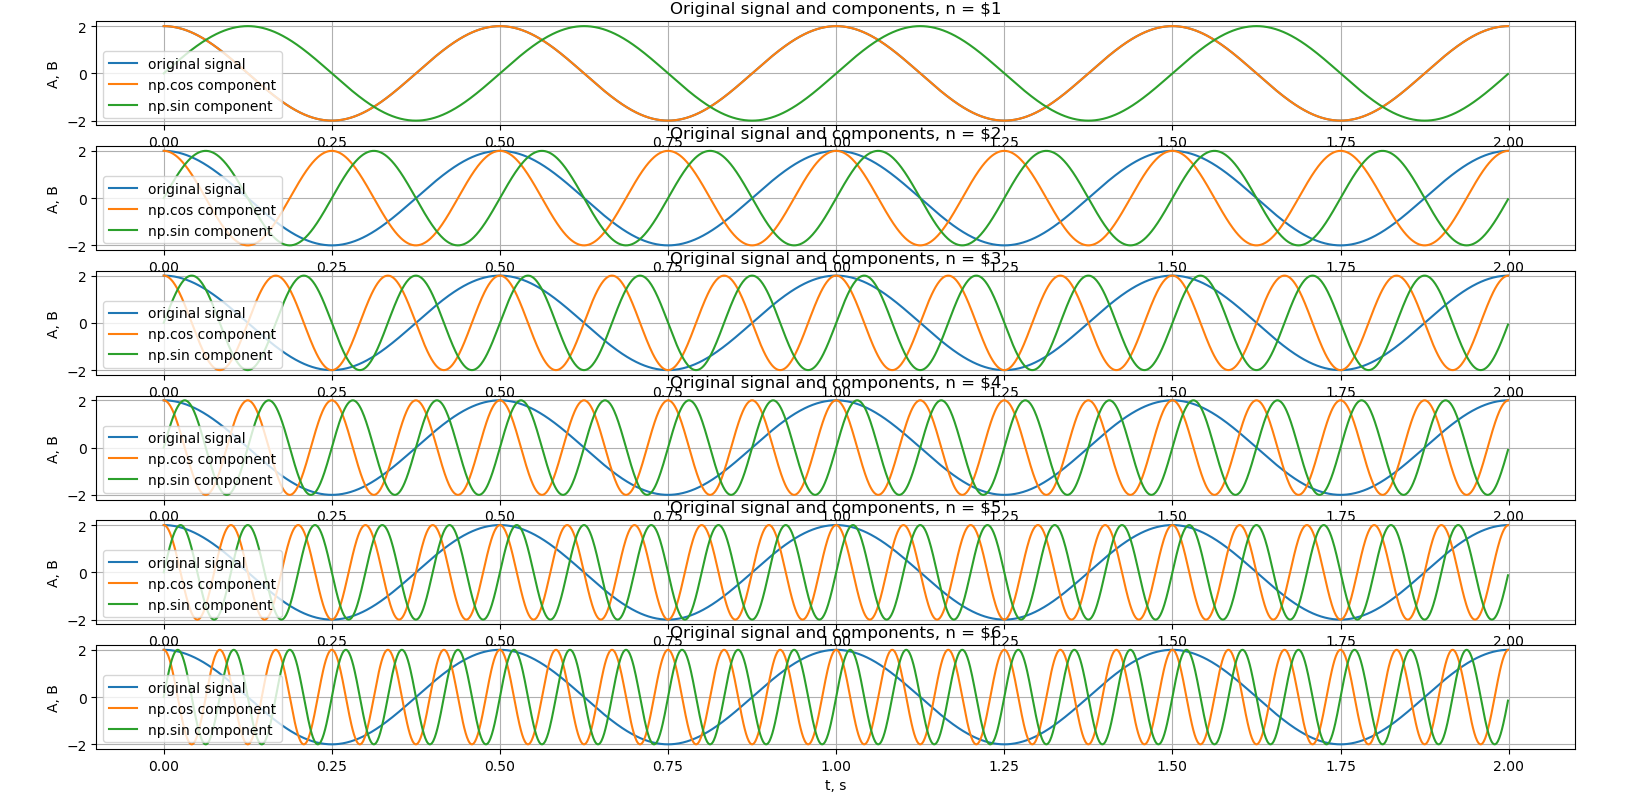
\includegraphics[width=1.0\textwidth]{task1_comp.png}
    \caption{Графики оригинального сигнала и компонент}
\end{figure}

\begin{figure}[H]
    \centering
    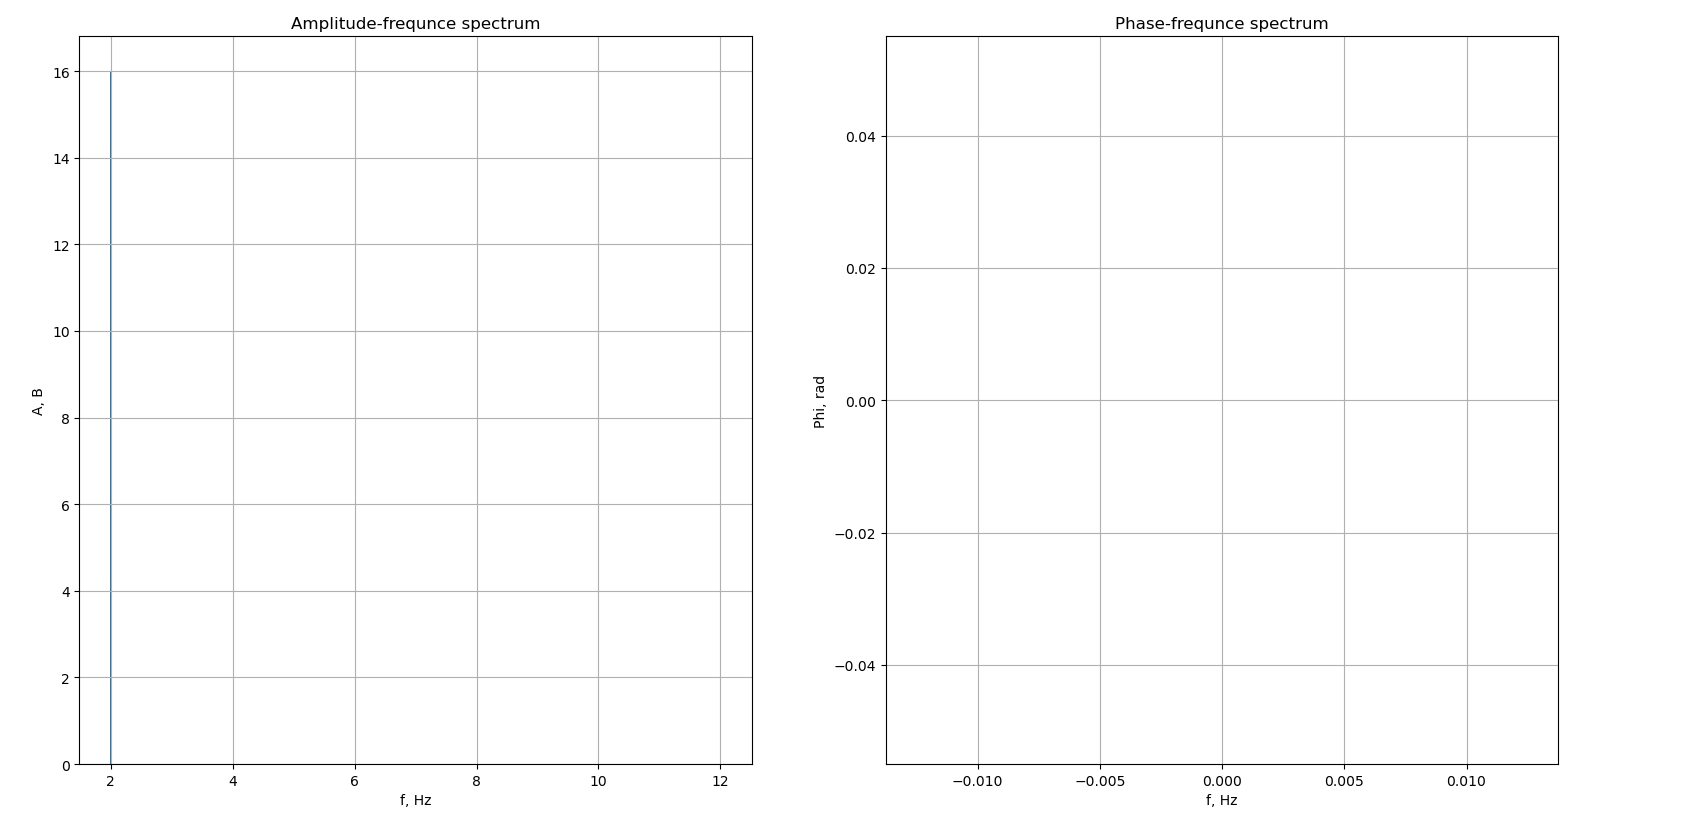
\includegraphics[width=1.0\textwidth]{task1_spec.png}
    \caption{АЧХ и ФЧХ сигнала}
\end{figure}

По АЧХ можем наблюдать, что в сигнале есть 1 компонента с часоттой 2Гц, именно такой сигнал
я изначально и задавал.

\subsection*{\textbf{Здание 2: простой сигнал с 2 компонентами с нулевой начальной фазой}}

Релизация задания в файле \textbf{task2.py} \\

Результат: \\

\begin{figure}[H]
    \centering
    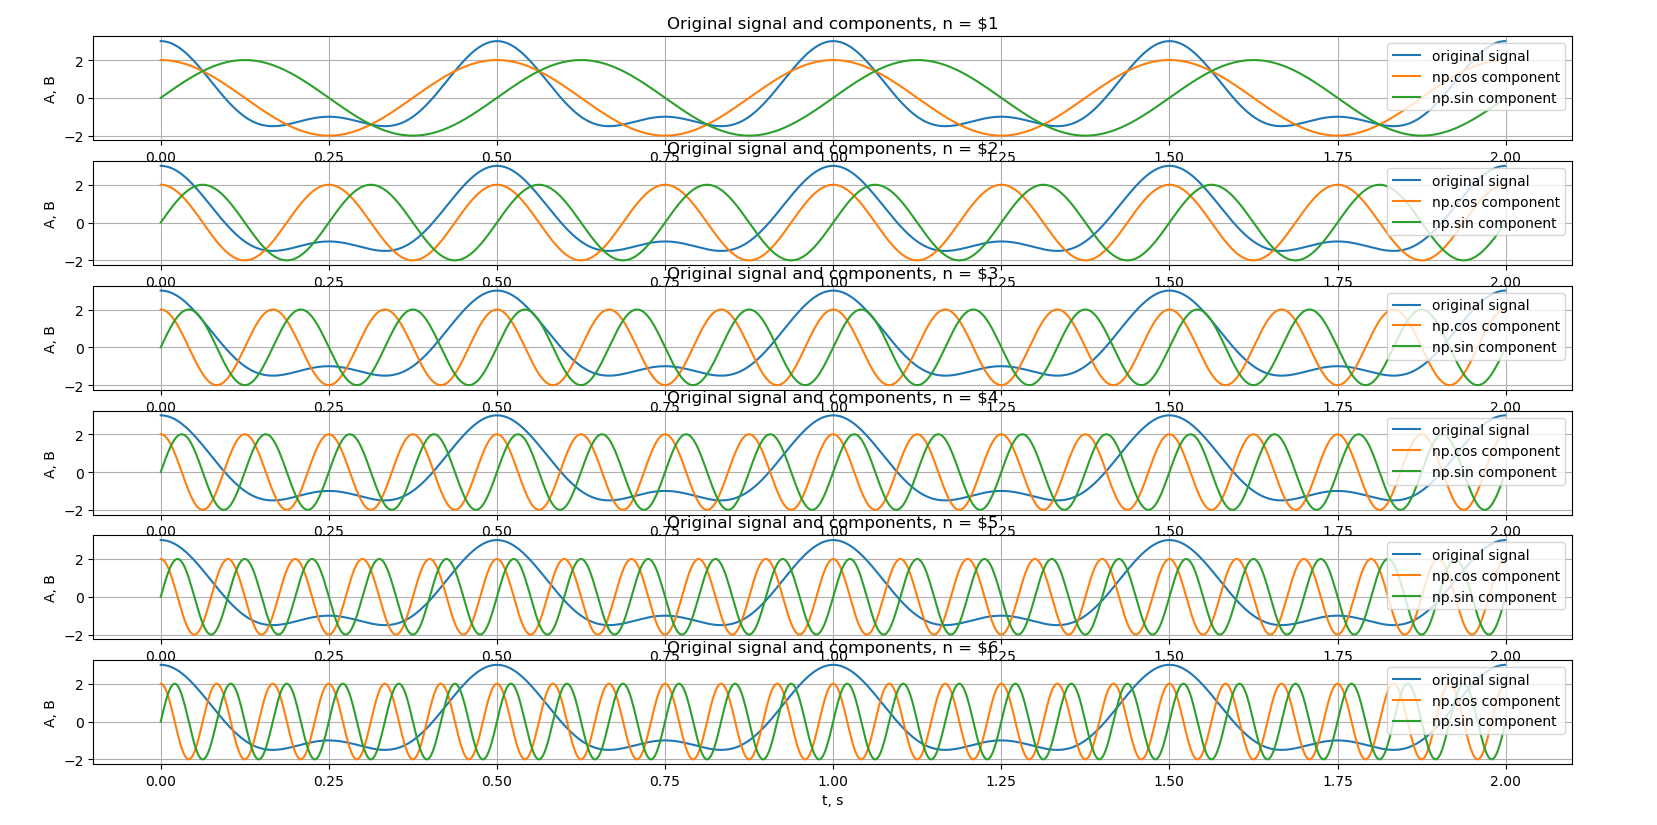
\includegraphics[width=1.0\textwidth]{task2_comp.png}
    \caption{Графики оригинального сигнала и компонент}
\end{figure}

\begin{figure}[H]
    \centering
    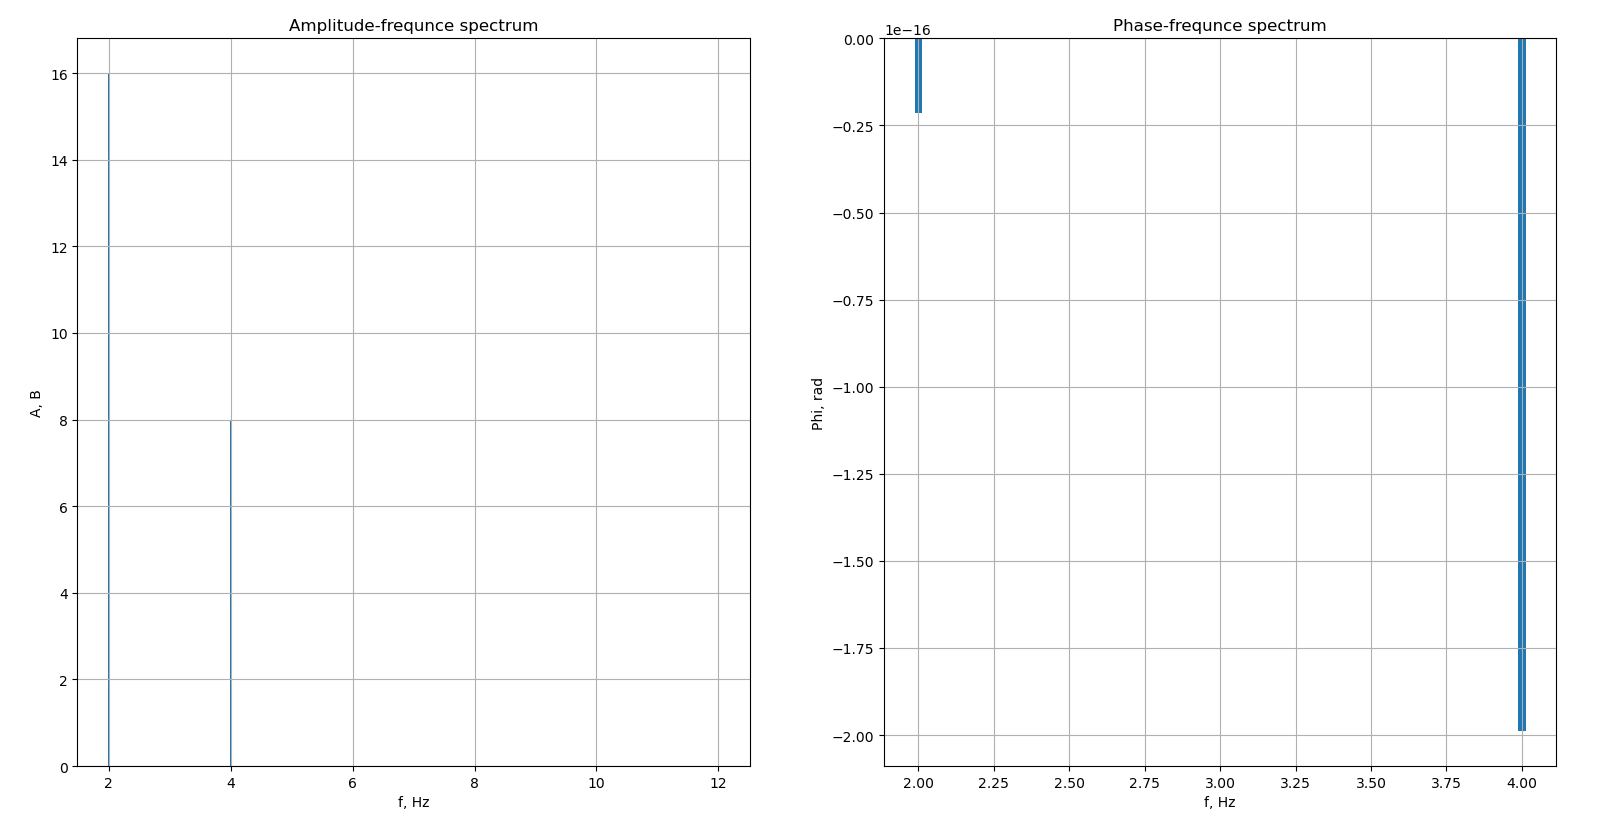
\includegraphics[width=1.0\textwidth]{task2_spec.png}
    \caption{АЧХ и ФЧХ сигнала}
\end{figure}

По АЧХ можем наблюдать, что в сигнале есть 2 компоненты с часоттой 2 и 4 Гц, именно такой сигнал
я изначально и задавал. На ФЧХ графике ложные фазы (это связано со свойствами acrtan).

\subsection*{\textbf{Здание 3: простой сигнал с 2 компонентами с ненулевой начальной фазой}}

Релизация задания в файле \textbf{task3.py} \\

Результат: \\

\begin{figure}[H]
    \centering
    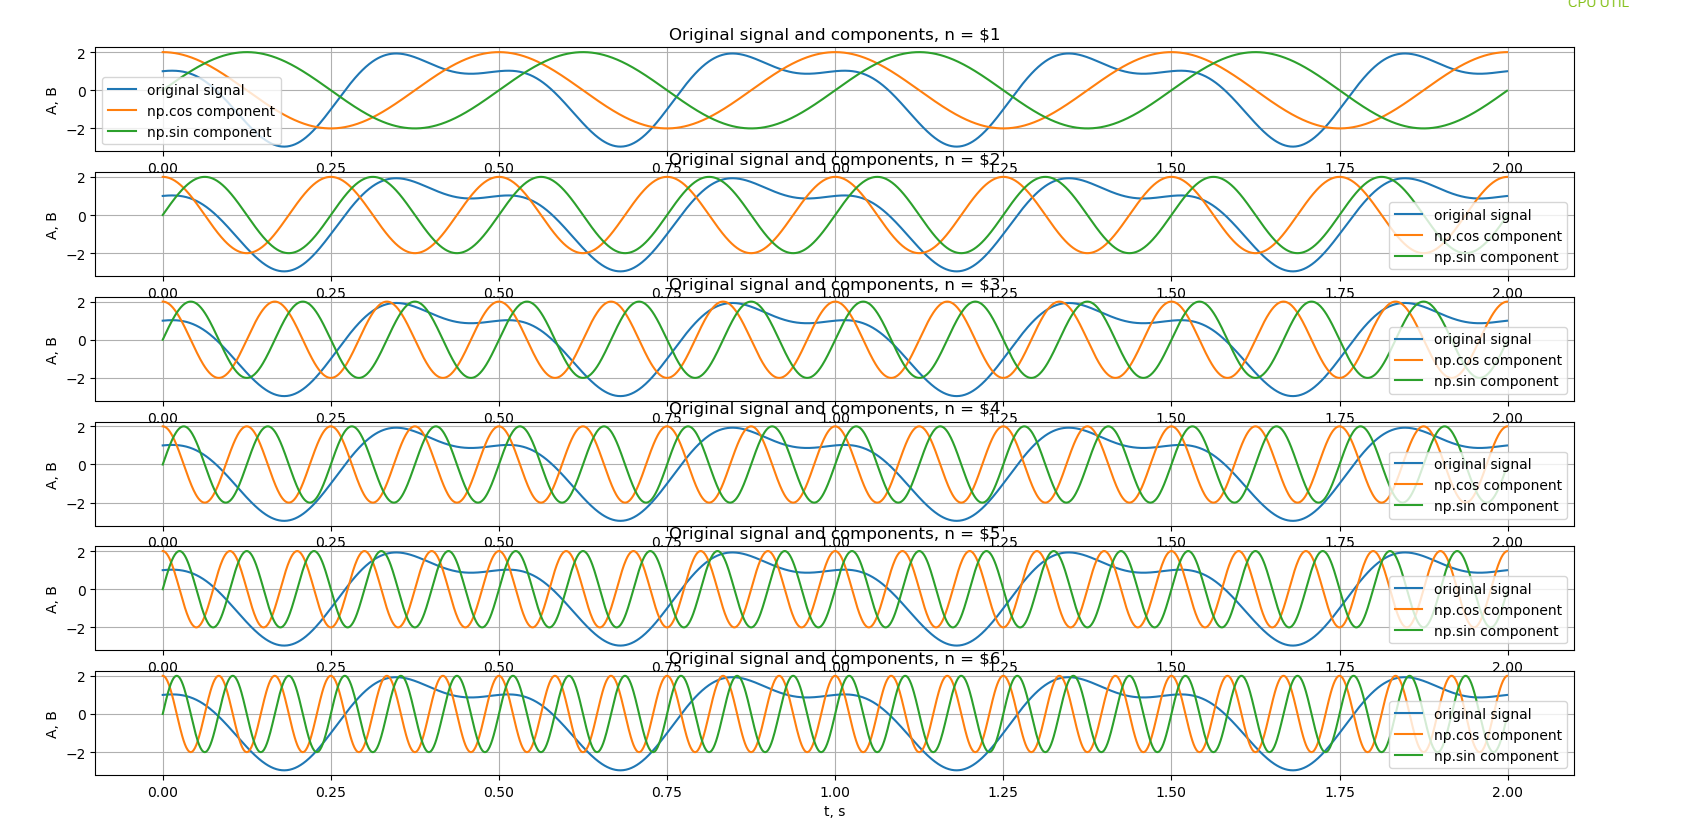
\includegraphics[width=1.0\textwidth]{task3_comp.png}
    \caption{Графики оригинального сигнала и компонент}
\end{figure}

\begin{figure}[H]
    \centering
    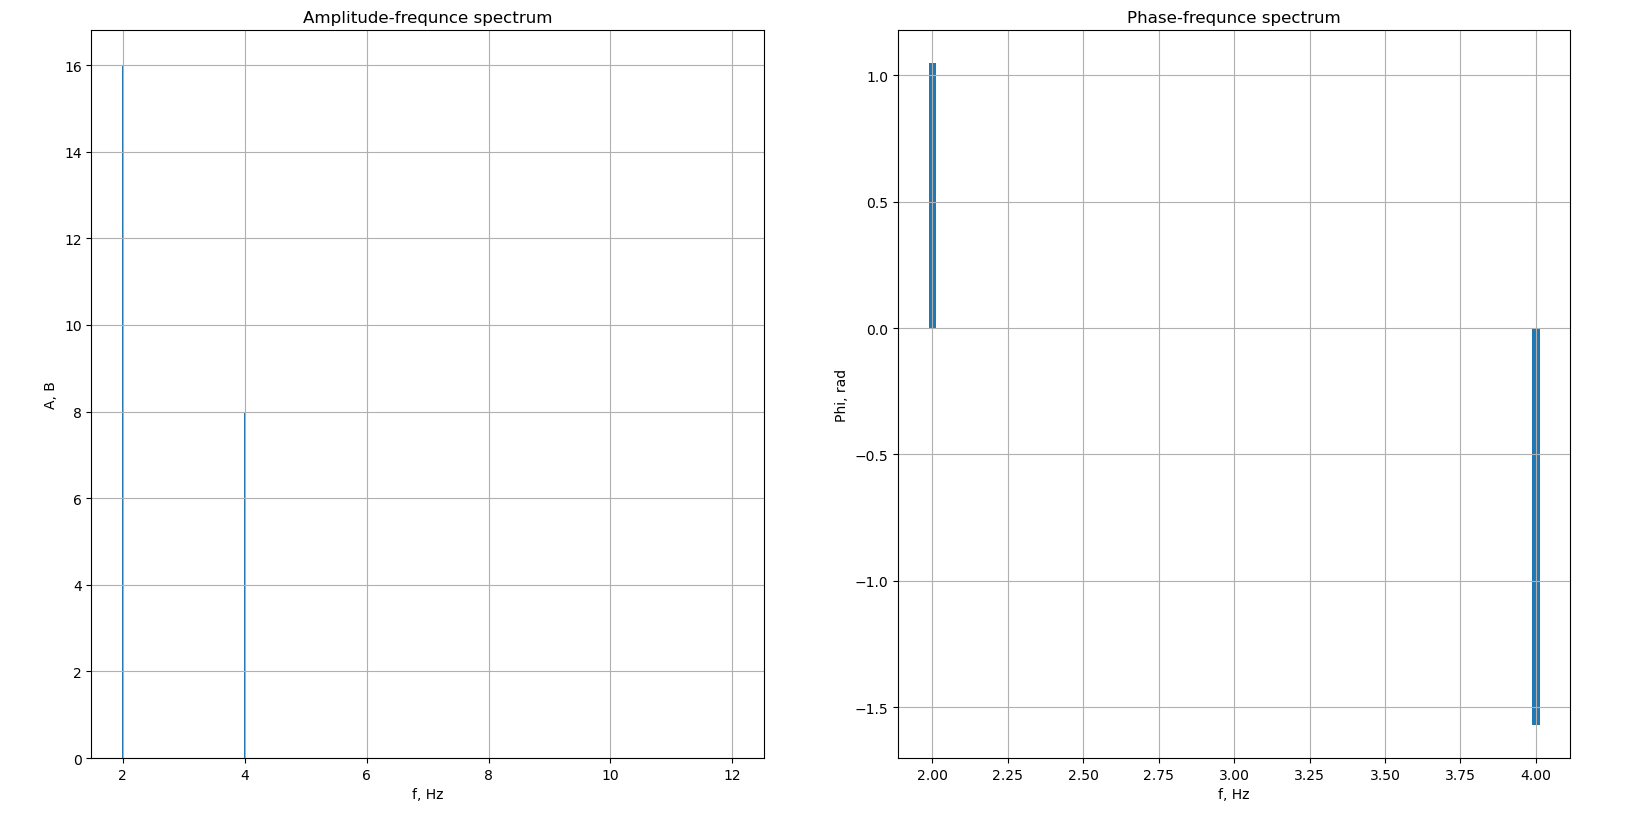
\includegraphics[width=1.0\textwidth]{task3_spec.png}
    \caption{АЧХ и ФЧХ сигнала}
\end{figure}

По АЧХ можем наблюдать, что в сигнале есть 2 компоненты с часоттой 2 и 4 Гц, именно такой сигнал
я изначально и задавал. На ФЧХ видим фазу $\pi/3$ для компоненты на 2Гц и $-\pi/3$ на 4 Гц, точно такой
сигнал я и задавал.

\subsection*{\textbf{Здание 4: прямоугольный сигнал}}

Релизация задания в файле \textbf{task4.py} \\

Результат: \\

\begin{figure}[H]
    \centering
    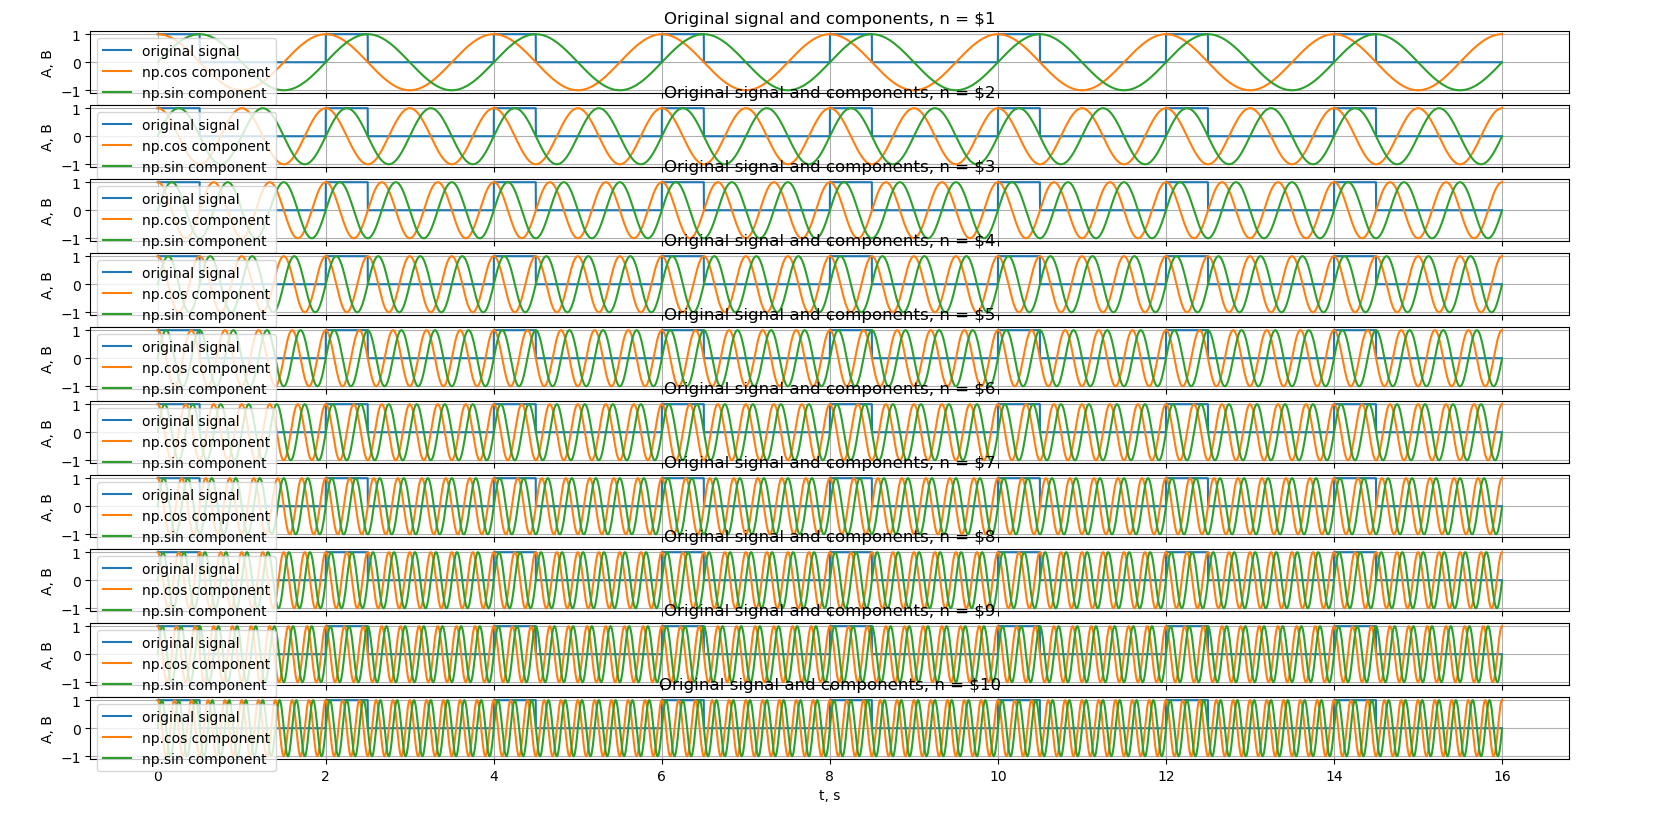
\includegraphics[width=1.0\textwidth]{task5_comp.png}
    \caption{Графики оригинального сигнала и компонент}
\end{figure}

\begin{figure}[H]
    \centering
    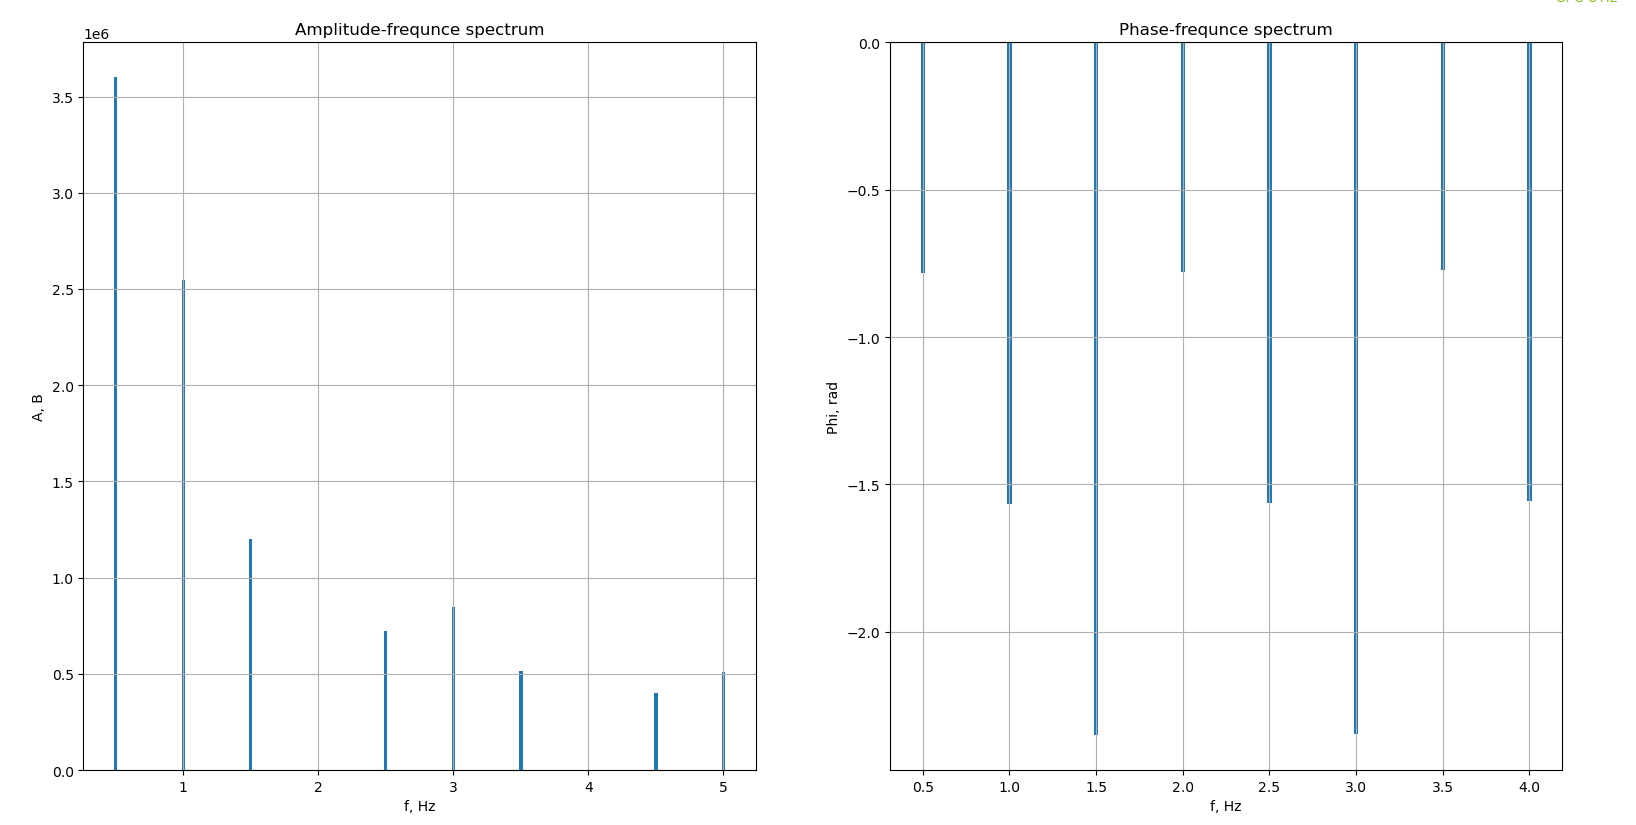
\includegraphics[width=1.0\textwidth]{task5_spectrum.png}
    \caption{АЧХ и ФЧХ сигнала}
\end{figure}

По АЧХ можем наблюдать, что в сигнале есть 2 компоненты с часоттой 2 и 4 Гц, именно такой сигнал
я изначально и задавал. На ФЧХ видим фазу $\pi/3$ для компоненты на 2Гц и $-\pi/3$ на 4 Гц, точно такой
сигнал я и задавал. \\

Теперь по полученным фазам и амплитудам попытаемся восстановить сигнал:

\begin{figure}[H]
    \centering
    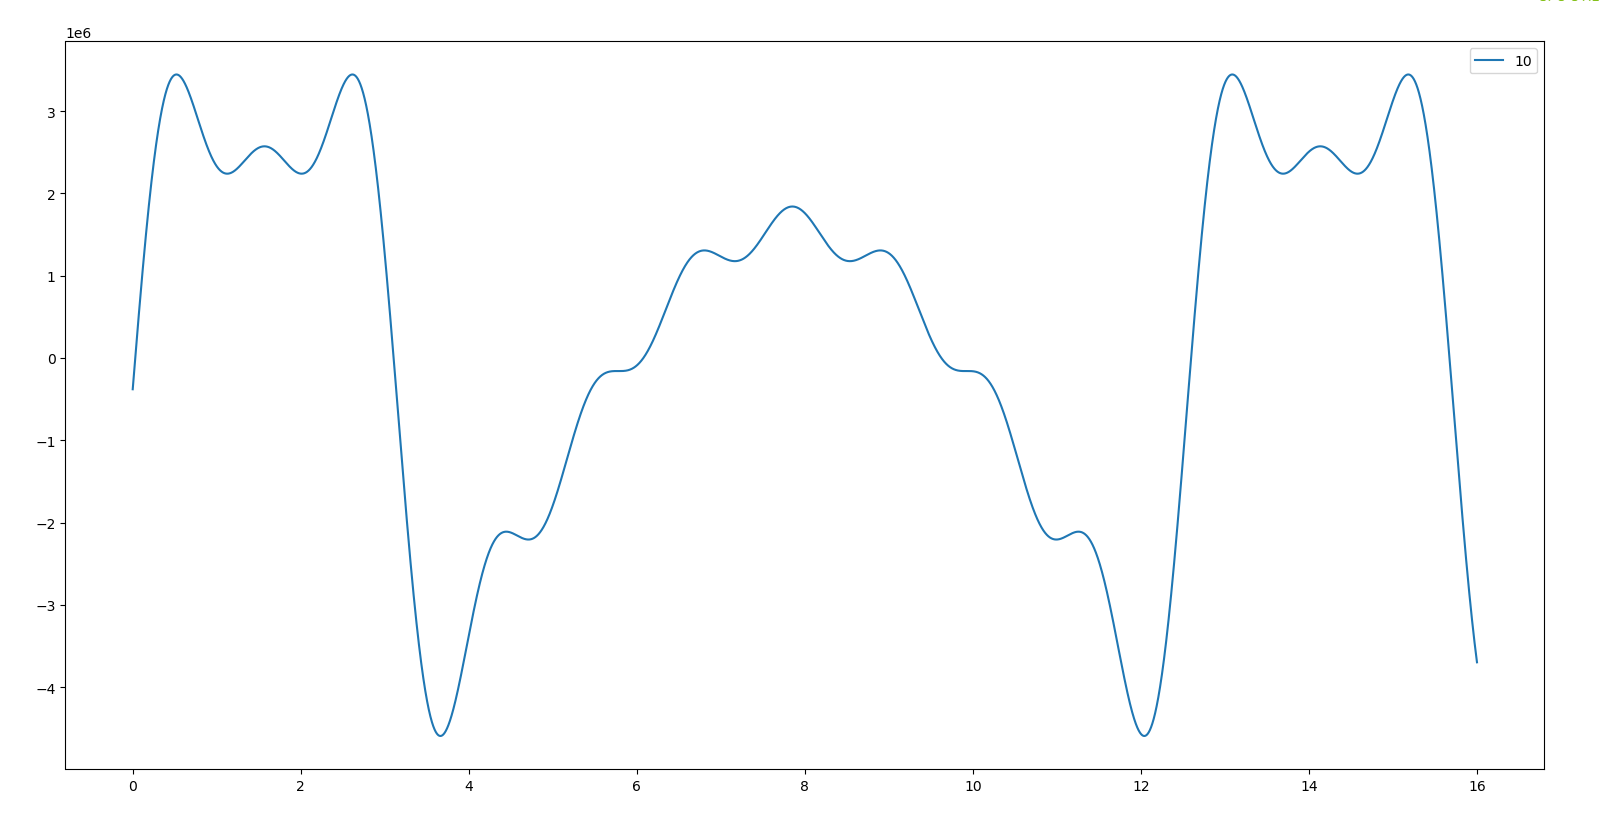
\includegraphics[width=1.0\textwidth]{ift.png}
    \caption{Пример восстановленного сигнала}
\end{figure}

Сигнал не очень похож на прямоугольный, но можно заметить, что по бокам он начинает приобретать прямоугольную форму.

\subsection*{\textbf{Здание 5: проверка ортогональности сигнала}}

Релизация задания в файле \textbf{task5.py} \\

Результат: \\

\begin{figure}[H]
    \centering
    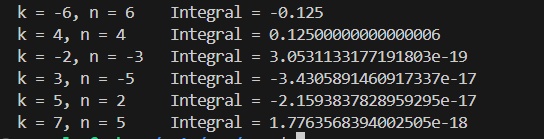
\includegraphics[width=1.0\textwidth]{task5_1.png}
    \caption{Проверка ортогональности при интегрировании по периоду}
\end{figure}

k и n - коэффициенты при частотах sin сигналов, у которых проверяется ортогональнось. \\

Заметим, что интеграл не равен нулю, когда n и k равны по модулю. Из этого можно сделать вывод о том, что 2 sin сигнала
ортогональны, если их частоты по модулю не равны. \\

Теперь сменим границы интегрирования. До этого интеграл был от 0 от Т, теперь будет от 0 до T+0.3:

\begin{figure}[H]
    \centering
    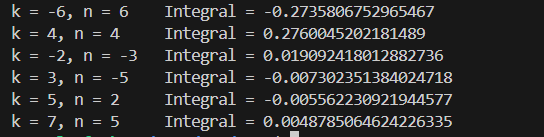
\includegraphics[width=1.0\textwidth]{task5_2.png}
    \caption{Проверка ортогональности при интегрировании не по периоду}
\end{figure}

Можем заметить, что интегралы ненулевые. Из этого следует, что ортогональность соблюдается только при рассмотрении сигналов
на периоде.

\textbf{Примечание:} целых нулевых значений не получилось из-за ошибок округления и прочего. Числа с $e^{-n}$ - машинный 0.



\endinput